% AA-34 | Audyt I, 22 XI 2026. Zrodlo po kontroli niezaleznej. Zachowano etykiety historyczne.
\chapter[Rezolwenta sześcienna i grupy Galois]{Rezolwenta sześcienna i grupy Galois wielomianów czwartego stopnia}\label{aa:ch:quartic-resolvent}

\section{Motywacja: skąd bierze się wielomian stopnia trzeciego?}
Niech $K$ będzie ciałem, $f\in K[X]$ wielomianem rozdzielczym
stopnia czwartego, a $G$ grupą Galois jego ciała rozkładu nad $K$.
Działa ona na czterech różnych pierwiastkach $f$.
Grupa $S_4$ działa nie tylko na czterech punktach, lecz również
na \emph{trzech} podziałach tych punktów na dwie pary.
Z tego działania otrzymamy wielomian stopnia trzeciego,
który pozwoli rozpoznać część informacji o $G$. Pierwiastkami
nowego wielomianu będą odpowiednie wyrażenia z pierwiastków $f$.

\section{Działanie na podziałach czteroelementowego zbioru}
\begin{definicja}\label{aa:def:quartic-pairings}
Niech $\Omega=\{1,2,3,4\}$. Przez $\mathcal P$ oznaczamy zbiór
trzech podziałów $\Omega$ na dwie nieuporządkowane pary:
\[
 P_1=\{\{1,2\},\{3,4\}\},\quad
 P_2=\{\{1,3\},\{2,4\}\},\quad
 P_3=\{\{1,4\},\{2,3\}\}.
\]
Dla $\sigma\in S_4$ i $P=\{\{i,j\},\{k,l\}\}$ definiujemy
$\sigma(P)=\{\{\sigma(i),\sigma(j)\},\{\sigma(k),\sigma(l)\}\}$.
Jest to działanie grupy $S_4$ na $\mathcal P$.
\end{definicja}

\begin{center}
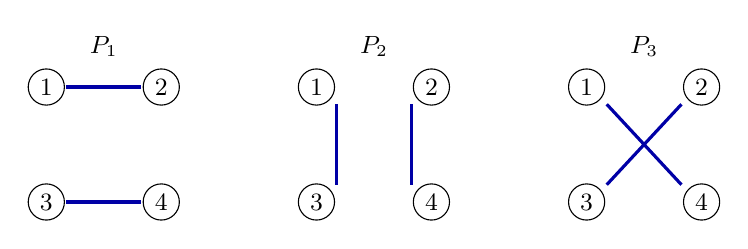
\begin{tikzpicture}[scale=.73, every node/.style={font=\small}]
\foreach \sh/\lab in {0/$P_1$,4.7/$P_2$,9.4/$P_3$}{
  \begin{scope}[xshift=\sh cm]
    \node at (1,2.7){\lab};
    \coordinate (a) at (0,2); \coordinate (b) at (2,2);
    \coordinate (c) at (0,0); \coordinate (d) at (2,0);
    \foreach \nm/\pt in {1/a,2/b,3/c,4/d}{\node[circle,draw,fill=white,inner sep=2pt] at (\pt) {\nm};}
  \end{scope}}
\begin{scope}[line width=1.15pt]
 \draw[blue!65!black] (0.35,2)--(1.65,2);
 \draw[blue!65!black] (0.35,0)--(1.65,0);
 \draw[blue!65!black] (5.05,1.7)--(5.05,.3);
 \draw[blue!65!black] (6.35,1.7)--(6.35,.3);
 \draw[blue!65!black] (9.75,1.7)--(11.05,.3);
 \draw[blue!65!black] (9.75,.3)--(11.05,1.7);
\end{scope}
\end{tikzpicture}
\end{center}
\begin{uwaga}
Na rysunku każdy odcinek łączy dwa elementy jednej pary.
Przecięcie odcinków w $P_3$ nie oznacza dodatkowego wierzchołka.
\end{uwaga}

\begin{twierdzenie}[Jądro działania na podziałach]\label{aa:tw:s4-v4}
Homomorfizm $\rho:S_4\to S(\mathcal P)\cong S_3$ jest surjektywny,
a jego jądro jest grupą Kleina
\[
 V_4=\{1,(12)(34),(13)(24),(14)(23)\}.
\]
W konsekwencji $S_4/V_4\cong S_3$.
\end{twierdzenie}
\begin{proof}
Permutacja $(12)$ ustala $P_1$ i zamienia $P_2$ z $P_3$.
Permutacja $(23)$ ustala $P_3$ i zamienia $P_1$ z $P_2$.
Zatem obraz $\rho$ zawiera transpozycje $(P_2\ P_3)$
oraz $(P_1\ P_2)$. Dwie sąsiednie transpozycje generują
całe $S(\mathcal P)$: ich iloczyny dają oba cykle długości trzy,
a ich sprzężenie daje trzecią transpozycję. To dowodzi surjektywności.
Każda z trzech podwójnych transpozycji zachowuje wszystkie trzy
podziały, co można sprawdzić, stosując podaną definicję działania.
Otrzymujemy więc $V_4\subseteq\ker\rho$. Z twierdzenia o homomorfizmie
$|\ker\rho|=|S_4|/|S_3|=24/6=4$.
Ponieważ $V_4$ ma dokładnie cztery elementy, jest całym jądrem.
\end{proof}

\section{Konstrukcja i jawne obliczenie rezolwenty}
\begin{definicja}\label{aa:def:quartic-resolvent}
Niech $K$ będzie ciałem, a
$f(X)=X^4+aX^3+bX^2+cX+d\in K[X]$ wielomianem monicznym.
Wybierzmy pierwiastki $\alpha_1,\ldots,\alpha_4$ wielomianu $f$
w pewnym ciele rozkładu, z uwzględnieniem krotności. Kładziemy
\[
 \beta_1=\alpha_1\alpha_2+\alpha_3\alpha_4,\quad
 \beta_2=\alpha_1\alpha_3+\alpha_2\alpha_4,\quad
 \beta_3=\alpha_1\alpha_4+\alpha_2\alpha_3.
\]
Wielomian $r_f(Y)=\prod_{i=1}^{3}(Y-\beta_i)$ nazywamy
\emph{rezolwentą sześcienną} $f$.
Zmiana numeracji $\alpha_i$ permutuje trzy wartości $\beta_i$,
więc nie zmienia samego wielomianu $r_f$.
\end{definicja}

\begin{twierdzenie}[Wzór na rezolwentę]\label{aa:tw:quartic-resolvent-formula}
Dla każdego ciała $K$ i każdego monicznego
$f=X^4+aX^3+bX^2+cX+d\in K[X]$ zachodzi
\[
 r_f(Y)=Y^3-bY^2+(ac-4d)Y-(a^2d+c^2-4bd).
\]
W szczególności $r_f\in K[Y]$ bez względu na charakterystykę $K$.
\end{twierdzenie}
\begin{proof}
Wprowadzamy elementarne funkcje symetryczne $e_1,e_2,e_3,e_4$
zmiennych $\alpha_1,\ldots,\alpha_4$. Ze wzorów Viète'a
(Twierdzenie~\ref{aa:tw:vieta-general}) otrzymujemy
$e_1=-a$, $e_2=b$, $e_3=-c$ oraz $e_4=d$.
Wyznaczymy kolejno trzy współczynniki $r_f$.

\emph{Suma pierwiastków.} W $\beta_1+\beta_2+\beta_3$
każdy iloczyn $\alpha_i\alpha_j$ ($i<j$) występuje dokładnie raz.
Zatem $\beta_1+\beta_2+\beta_3=e_2$.

\emph{Suma iloczynów parami.} Na przykład
\[
\begin{aligned}
 \beta_1\beta_2={}&\alpha_1^2\alpha_2\alpha_3
 +\alpha_1\alpha_2^2\alpha_4
 +\alpha_1\alpha_3^2\alpha_4
 +\alpha_2\alpha_3\alpha_4^2.
\end{aligned}
\]
Dwa pozostałe iloczyny powstają przez permutacje indeksów.
Łącznie otrzymujemy wszystkie $12$ jednomianów postaci
$\alpha_i^2\alpha_j\alpha_k$, gdzie $i,j,k$ są parami różne,
każdy dokładnie raz. Z kolei w $e_1e_3$ powstają te same
$12$ jednomianów oraz $4e_4$: w iloczynie $\alpha_i$ z sumą
czterech jednomianów trzeciego stopnia jeden z nich nie zawiera
$\alpha_i$, a pozostałe trzy go zawierają.
Stąd $\sum_{i<j}\beta_i\beta_j=e_1e_3-4e_4$.

\emph{Iloczyn trzech pierwiastków.} Oznaczmy
$T_i=\prod_{j\ne i}\alpha_j$ dla $1\le i\le4$.
Po wymnożeniu trzech nawiasów $\beta_1\beta_2\beta_3$
dostajemy osiem jednomianów: cztery postaci $T_i^2$ i cztery
postaci $e_4\alpha_i^2$. Dlatego
\[
 \beta_1\beta_2\beta_3=\sum_{i=1}^4 T_i^2
 +e_4\sum_{i=1}^4\alpha_i^2.
\]
Z tożsamości
$e_1^2=\sum_i\alpha_i^2+2e_2$ wynika
$\sum_i\alpha_i^2=e_1^2-2e_2$.
Ponieważ $T_iT_j=e_4\alpha_k\alpha_l$ dla
$\{i,j,k,l\}=\{1,2,3,4\}$,
mamy też
$e_3^2=\sum_iT_i^2+2e_4e_2$.
Po podstawieniu i zebraniu wyrazów otrzymujemy
\[
 \beta_1\beta_2\beta_3=e_1^2e_4+e_3^2-4e_2e_4.
\]
Wszystkie te równości są tożsamościami wielomianowymi
o współczynnikach całkowitych, więc obowiązują również w
charakterystyce $2$ i $3$. Zastępując $e_i$ przez współczynniki
$f$ oraz stosując wzory Viète'a do $r_f$, dostajemy tezę.
\end{proof}

\begin{twierdzenie}[Rezolwenta i grupa Galois]\label{aa:tw:quartic-resolvent-action}
Niech $K$ będzie ciałem charakterystyki różnej od $2$,
a $f\in K[X]$ monicznym, rozdzielczym wielomianem stopnia czwartego.
Niech $L$ będzie ciałem rozkładu $f$, a $G=\operatorname{Gal}(L/K)$
traktujmy jako podgrupę $S_4$ przez działanie na
$\alpha_1,\ldots,\alpha_4$. Wówczas $\beta_1,\beta_2,\beta_3$
są parami różne, a grupa Galois rezolwenty jest izomorficzna
z $\rho(G)\le S_3$. Jądrem działania $G$ na pierwiastkach
rezolwenty jest $G\cap V_4$.
\end{twierdzenie}
\begin{proof}
Wprost z definicji mamy
\[
 \beta_1-\beta_2=(\alpha_1-\alpha_4)(\alpha_2-\alpha_3),\quad
 \beta_1-\beta_3=(\alpha_1-\alpha_3)(\alpha_2-\alpha_4),
\]
a różnicę $\beta_2-\beta_3$ otrzymujemy analogicznie.
Ponieważ wielomian $f$ jest rozdzielczy, każda różnica
dwóch różnych $\alpha_i$ jest niezerowa. Ciało nie ma dzielników
zera, więc również $\beta_i\ne\beta_j$ dla $i\ne j$.

Dla $\sigma\in G$ zachodzi $\sigma(\beta_i)=\beta_j$ dokładnie
wtedy, gdy $\sigma$ wysyła podział $P_i$ na $P_j$.
Ponieważ $\beta_i$ są różne, oba działania mają to samo jądro:
$G\cap\ker\rho=G\cap V_4$.
Ciało $M=K(\beta_1,\beta_2,\beta_3)$ jest ciałem rozkładu
$r_f$ zawartym w $L$. Zatem $M/K$ jest rozszerzeniem Galois.
Ograniczenie automorfizmów $L/K$ do $M/K$ jest surjektywne
na mocy odpowiedniości Galois, a jego jądrem jest $G\cap V_4$.
Twierdzenie o izomorfizmie daje
$\operatorname{Gal}(M/K)\cong G/(G\cap V_4)\cong\rho(G)$.
\end{proof}

\begin{wniosek}[Równość wyróżników]\label{aa:wn:quartic-resolvent-disc}
Niech $K$ będzie dowolnym ciałem, a $f\in K[X]$ monicznym
wielomianem stopnia czwartego. Dla rezolwenty $r_f$ z
Definicji~\ref{aa:def:quartic-resolvent} zachodzi
\[
\operatorname{disc}(r_f)=\operatorname{disc}(f).
\]
W szczególności $f$ jest rozdzielczy wtedy i tylko wtedy,
gdy $r_f$ jest rozdzielczy.
\end{wniosek}
\begin{proof}
Dla pierwiastków $\alpha_1,\ldots,\alpha_4$ wielomianu $f$,
uwzględnionych z krotnościami, mamy
\[
\begin{aligned}
\beta_1-\beta_2&=(\alpha_1-\alpha_4)(\alpha_2-\alpha_3),\\
\beta_1-\beta_3&=(\alpha_1-\alpha_3)(\alpha_2-\alpha_4),\\
\beta_2-\beta_3&=(\alpha_1-\alpha_2)(\alpha_3-\alpha_4).
\end{aligned}
\]
Po pomnożeniu kwadratów tych trzech równości otrzymujemy
dokładnie sześć czynników tworzących definicję
$\operatorname{disc}(f)$. Jest to tożsamość wielomianowa,
ważna także w charakterystyce $2$ i dla pierwiastków
wielokrotnych. Ostatnie stwierdzenie wynika z
Twierdzenia~\ref{aa:tw:disc-separable}.
\end{proof}

\begin{uwaga}\label{aa:uw:quartic-char2}
Równości dla $\beta_i-\beta_j$ są poprawne także w charakterystyce
$2$. Zatem rozdzielczy $f$ ma trzy różne pierwiastki rezolwenty
również w tej charakterystyce, a opis obrazu $\rho(G)$ pozostaje
prawdziwy. Ograniczenie $\operatorname{char}K\ne2$ jest natomiast
konieczne przy późniejszym wykorzystaniu kryterium wyróżnika
z Twierdzenia~\ref{aa:tw:disc-alternating}.
\end{uwaga}

\section{Możliwe grupy dla nierozkładalnego wielomianu}
\begin{twierdzenie}[Przypadek nierozkładalny]\label{aa:tw:quartic-classification}
Niech $K$ będzie ciałem charakterystyki różnej od $2$,
a $f\in K[X]$ monicznym, nierozkładalnym i rozdzielczym
wielomianem stopnia czwartego. Wtedy jego grupa Galois
jest izomorficzna z jedną z grup $C_4$, $V_4$, $D_4$, $A_4$, $S_4$.
Jeżeli ponadto $r_f$ jest nierozkładalny nad $K$, to
$G\cong A_4$ albo $G\cong S_4$; w takim przypadku
$G\cong A_4$ dokładnie wtedy, gdy $\operatorname{disc}(f)$
jest kwadratem niezerowego elementu $K$.
\end{twierdzenie}
\begin{proof}
Ponieważ $f$ jest nierozkładalny i rozdzielczy, grupa Galois
działa przechodnio na czterech jego pierwiastkach.
Dla jednego pierwiastka $\alpha_1$ twierdzenie o orbicie
i stabilizatorze daje $|G|=4|G_{\alpha_1}|$.
Jako podgrupa $S_4$ grupa $G$ ma rząd dzielący $24$,
więc $|G|$ należy do $\{4,8,12,24\}$.

Jeżeli $|G|=4$, stabilizator pierwiastka jest trywialny,
a działanie jest regularne. Grupa rzędu cztery jest albo
cykliczna $C_4$ (gdy zawiera element rzędu cztery), albo
izomorficzna z $V_4$ (gdy każdy nietrywialny element ma rząd dwa).
W drugim przypadku każdy element $z\in G$ spełnia $z^2=1$.
Dla dowolnych $x,y\in G$ mamy więc
$(xy)^{-1}=xy$, a jednocześnie $(xy)^{-1}=y^{-1}x^{-1}=yx$.
Stąd $xy=yx$, co potwierdza przemienność. Argument obejmuje
także przypadki $x=y$ oraz $x=1$ lub $y=1$.

Jeżeli $|G|=8$, grupa $G$ jest podgrupą Sylowa rzędu $8$
w $S_4$. Grupa symetrii kwadratu wpisanego w cztery wierzchołki
ma osiem elementów: generują ją obrót $(1234)$ i odbicie $(24)$
z relacjami $r^4=s^2=1$, $srs=r^{-1}$.
Na mocy twierdzenia Sylowa każda podgrupa rzędu $8$
jest z nią sprzężona, zatem izomorficzna z $D_4$.

Jeżeli $|G|=12$, podgrupa $G$ ma indeks dwa i jest normalna.
Działanie $S_4$ na dwóch warstwach $S_4/G$ daje
nietrywialny homomorfizm $S_4\to C_2$ z jądrem $G$.
Każda transpozycja ma taki sam obraz, bo transpozycje są sprzężone.
Obraz ten nie może być tożsamością, gdyż transpozycje generują
$S_4$. Homomorfizm jest więc znakiem permutacji, a $G=A_4$.
Jeżeli $|G|=24$, to $G=S_4$.

Załóżmy teraz, że rezolwenta jest nierozkładalna. Z poprzedniego
twierdzenia wiemy, że jej grupa Galois działa przechodnio
na trzech pierwiastkach; ma więc rząd podzielny przez $3$.
Jest ona obrazem $G$, toteż $3\mid |G|$.
Wśród rozpatrywanych rzędów $4,8,12,24$ warunek ten
spełniają tylko $12$ i $24$. Pozostają grupy $A_4$ i $S_4$.
Ponieważ $\operatorname{char}K\ne2$, kryterium wyróżnika
z Twierdzenia~\ref{aa:tw:disc-alternating} mówi, że
$G\le A_4$ dokładnie wtedy, gdy wyróżnik jest kwadratem w $K$.
Rozdzielczość $f$ gwarantuje, że wyróżnik jest niezerowy.
\end{proof}

\begin{wniosek}[Rozkład rezolwenty a grupa Galois]
\label{aa:wn:quartic-resolvent-factorization}
Niech $K$ będzie ciałem charakterystyki różnej od $2$,
a $f\in K[X]$ monicznym, nierozkładalnym i rozdzielczym
wielomianem stopnia czwartego. Wówczas rezolwenta $r_f$
jest rozdzielcza i zachodzi dokładnie jeden z trzech przypadków:
\begin{enumerate}
\item jeśli $r_f$ rozkłada się na trzy czynniki liniowe w $K[Y]$,
      to $\operatorname{Gal}(f/K)\cong V_4$;
\item jeśli $r_f$ ma jeden czynnik liniowy i jeden nierozkładalny
      czynnik kwadratowy, to $\operatorname{Gal}(f/K)\cong C_4$
      albo $D_4$;
\item jeśli $r_f$ jest nierozkładalna, to
      $\operatorname{Gal}(f/K)\cong A_4$ albo $S_4$.
\end{enumerate}
W ostatnim przypadku wyróżnik $f$ rozstrzyga między $A_4$
i $S_4$ zgodnie z Twierdzeniem~\ref{aa:tw:quartic-classification}.
\end{wniosek}
\begin{proof}
Z Twierdzenia~\ref{aa:tw:quartic-resolvent-action} pierwiastki
$r_f$ są różne, a działanie jej grupy Galois to obraz
$\rho(G)\subseteq S_3$, gdzie $G=\operatorname{Gal}(f/K)$.
Trzy typy rozkładu odpowiadają odpowiednio orbitom
$1+1+1$, $1+2$ i $3$ na zbiorze trzech pierwiastków.
W pierwszym przypadku $\rho(G)=1$, zatem $G\subseteq V_4$;
z przechodniości $G$ na czterech pierwiastkach $f$ wynika
$4\mid |G|$, więc $G=V_4$. W drugim przypadku obraz
ma rząd $2$. Na mocy klasyfikacji w
Twierdzeniu~\ref{aa:tw:quartic-classification} może być wtedy
tylko $C_4$ albo $D_4$: obie te grupy mają obraz rzędu $2$,
podczas gdy $V_4$ ma obraz trywialny, $A_4$ obraz rzędu $3$,
a $S_4$ obraz rzędu $6$.
Trzeci przypadek jest już drugą częścią wspomnianego twierdzenia.
Ponieważ rozdzielcza rezolwenta stopnia trzeciego ma tylko
wymienione typy rozkładu, lista jest wyczerpująca.
\end{proof}

\begin{przyklad}[Cykliczna grupa $C_4$]\label{aa:prz:quartic-c4}
Niech $f(X)=\Phi_5(X)=X^4+X^3+X^2+X+1\in\mathbb Q[X]$.
Po podstawieniu $X=T+1$ otrzymujemy
\[
 f(T+1)=T^4+5T^3+10T^2+10T+5.
\]
Kryterium Eisensteina dla liczby pierwszej $5$ dowodzi
nierozkładalności $f$ nad $\mathbb Q$.
Ciałem rozkładu $f$ jest $\mathbb Q(\zeta_5)$, a grupa Galois
jest izomorficzna z
$(\mathbb Z/5\mathbb Z)^\times\cong C_4$;
izomorfizm ten wynika z
Twierdzenia~\ref{aa:tw:cyclotomic-galois}.
Z Twierdzenia~\ref{aa:tw:quartic-resolvent-formula},
przy $a=b=c=d=1$, mamy
\[
 r_f(Y)=Y^3-Y^2-3Y+2=(Y-2)(Y^2+Y-1).
\]
Czynnik kwadratowy jest nierozkładalny nad $\mathbb Q$,
gdyż jego wyróżnik wynosi $5$, niebędące kwadratem
liczby wymiernej. Jest to przypadek $1+2$ poprzedniego
wniosku. Pokazuje on również, że rozkład $1+2$
rezolwenty nie wystarcza do rozróżnienia grup $C_4$ i $D_4$.
\end{przyklad}

\begin{przyklad}[Grupa $S_4$]\label{aa:prz:quartic-s4}
Weźmy $f=X^4-X-1\in\mathbb Q[X]$. Współczynniki
$a=b=0$, $c=d=-1$ dają rezolwentę
$r_f(Y)=Y^3+4Y-1$.
Ponieważ jest ona moniczna o współczynnikach całkowitych,
każdy jej pierwiastek wymierny musiałby należeć do $\{1,-1\}$.
Tymczasem $r_f(1)=4$ i $r_f(-1)=-6$,
więc $r_f$ jest nierozkładalny jako wielomian sześcienny.

Redukcja $f$ modulo $2$ jest równa $X^4+X+1$.
Nie ma pierwiastka w $\mathbb F_2$ (wartości w $0,1$ wynoszą $1$),
a jedyny moniczny nierozkładalny wielomian kwadratowy
nad $\mathbb F_2$ to $X^2+X+1$.
Jego kwadrat wynosi $X^4+X^2+1$, a nie $X^4+X+1$.
Gdyby nasz wielomian stopnia czwartego był rozkładalny,
miałby czynnik liniowy lub dwa czynniki nierozkładalne stopnia dwa;
oba przypadki są wykluczone. Zatem $f$ jest nierozkładalny nad
$\mathbb F_2$, a w konsekwencji nad $\mathbb Q$.

Wyróżnik monicznego wielomianu $X^4+cX+d$ można obliczyć
jako wypadkową z pochodną $4X^3+c$.
Jeśli $t^3=-c/4$, to
$t^4+ct+d=d+(3c/4)t$, więc iloczyn wartości
$f(t)$ po trzech pierwiastkach pochodnej jest
$d^3-27c^4/256$: dla pierwiastków $t_1,t_2,t_3$
wielomianu $X^3+c/4$ mamy $\sum_i t_i=0$,
$\sum_{i<j}t_it_j=0$ i $t_1t_2t_3=-c/4$.
Wzór na wypadkową daje
$R(f',f)=4^4\prod_i f(t_i)$, zaś symetria wypadkowej
(Twierdzenie~\ref{aa:wn:res-sym}) daje
$R(f,f')=R(f',f)$, bo $4\cdot3$ jest parzyste.
Otrzymujemy
$\operatorname{disc}(X^4+cX+d)=256d^3-27c^4$.
Dla $c=d=-1$ jest to $-283$, liczba ujemna, a zatem
niekwadrat w $\mathbb Q$. Na mocy
Twierdzenia~\ref{aa:tw:quartic-classification} mamy
$\operatorname{Gal}(f/\mathbb Q)\cong S_4$.
\end{przyklad}

\begin{przyklad}[Kontrprzykład: rezolwenta rozkładalna, a wielomian nierozkładalny]\label{aa:prz:quartic-v4}
Wielomian $f=X^4-2$ jest nierozkładalny nad $\mathbb Q$
na mocy kryterium Eisensteina dla liczby pierwszej $2$.
Wzór na rezolwentę daje
$r_f(Y)=Y^3+8Y=Y(Y^2+8)$, więc rezolwenta jest rozkładalna.
Niech $\alpha=\sqrt[4]{2}>0$. Ciało rozkładu jest
$L=\mathbb Q(\alpha,i)$, ponieważ pierwiastki $f$
to $\alpha,-\alpha,i\alpha,-i\alpha$.
Mamy $[\mathbb Q(\alpha):\mathbb Q]=4$, a
$\mathbb Q(\alpha)\subset\mathbb R$, zatem $i\notin\mathbb Q(\alpha)$
i $[L:\mathbb Q]=8$.
Ponieważ $[L:\mathbb Q(i)]=8/2=4$, minimalnym
wielomianem $\alpha$ nad $\mathbb Q(i)$ jest $X^4-2$.
Liczba $i\alpha$ jest również jego pierwiastkiem, dlatego
$\mathbb Q(i)$-zanurzenie wyznaczone przez
$\alpha\mapsto i\alpha$ jest automorfizmem $L$.
Oznaczmy je przez $r$. Automorfizm ten ustala $i$,
a sprzężenie zespolone $s$ ustala $\alpha$ i wysyła
$i$ na $-i$. Spełniają one relacje
$r^4=s^2=1$, $srs=r^{-1}$, a osiem automorfizmów
$r^k,sr^k$ ($0\le k<4$) jest różnych.
Grupa Galois ma więc postać $D_4$ i nie jest ani $A_4$, ani $S_4$.
Przykład pokazuje, dlaczego w drugiej części
Twierdzenia~\ref{aa:tw:quartic-classification} trzeba
zakładać nierozkładalność rezolwenty.
\end{przyklad}

\begin{przyklad}[Grupa Kleina i całkowicie rozkładalna rezolwenta]\label{aa:prz:quartic-klein}
Niech $\alpha=\sqrt2+\sqrt3$ oraz
$f=X^4-10X^2+1$. Ponieważ $\alpha^2=5+2\sqrt6$,
liczba $\alpha$ spełnia $(\alpha^2-5)^2=24$,
czyli $f(\alpha)=0$.
Ponadto $\alpha^{-1}=\sqrt3-\sqrt2$, skąd
\[
 \sqrt2=\frac{\alpha-\alpha^{-1}}2,\qquad
 \sqrt3=\frac{\alpha+\alpha^{-1}}2.
\]
Zatem $\mathbb Q(\alpha)=\mathbb Q(\sqrt2,\sqrt3)$.
Jest to rozszerzenie stopnia czwartego: $\sqrt3$ nie należy
do $\mathbb Q(\sqrt2)$, bo równość
$(u+v\sqrt2)^2=3$ dla $u,v\in\mathbb Q$
wymagałaby $uv=0$ i następnie $u^2=3$ lub $v^2=3/2$,
co jest niemożliwe dla liczb wymiernych.
Wobec tego $f$ jest nierozkładalny.
Jego pierwiastki to $\pm\sqrt2\pm\sqrt3$, wszystkie należą
do $\mathbb Q(\sqrt2,\sqrt3)$. Grupa Galois jest więc $V_4$:
niezależnie można zmieniać znaki obu pierwiastków kwadratowych.
Wzór z Twierdzenia~\ref{aa:tw:quartic-resolvent-formula} daje
\[
 r_f(Y)=Y^3+10Y^2-4Y-40=(Y+10)(Y-2)(Y+2).
\]
Wszystkie trzy pierwiastki rezolwenty są wymierne,
co odpowiada trywialnemu obrazowi $V_4$ w $S_3$.
\end{przyklad}
